Managing complex data flows and update patterns is one of the most difficult challenges in interactive data visualization. Constructing interactive visualizations with multiple linked views can be a daunting task. Functional reactive programming provides approaches for specifying data dependency graphs declaratively and maintaining them automatically. Functional reactive programming can be combined with the Model View Controller (MVC) paradigm to provide reactive models, an effective abstraction that supports construction of complex interactive data visualization systems.

Even with the wealth of visualization toolkits and libraries that exist today, there is a need for an abstraction that addresses the core issue of managing complex data flows and update propagation patterns. In this chapter, a novel approach for developing reusable interactive visualization components using reactive models (reactive visualizations) is introduced. A pseudocode implementation of reactive models is presented in appendix A. A JavaScript implementation of reactive models has been released as the open source ModelJS project \cite{modeljs}. The effectiveness of the proposed approach is demonstrated in several visualization examples including multiple linked views.

\section{Related Work}
The first attempt at a systematic formalization of data visualization was Jacques Bertin's ``Semiology of Graphics'' \cite{bertin1983semiology}. In this work, Bertin relates data types to visual marks and channels in a coherent system that takes visual perception into account. Bertin's work has influenced many future theoretical underpinnings of visualization, including Leland Wilkinson's ``Grammar of Graphics'' \cite{wilkinson2005grammar} and Jock Mackinlay's APT (A Presentation Tool) system \cite{mackinlay1986automating}, which led to the development of the commercial visualization package Tableau \cite{hanrahan2007visual}.

Interactions within data visualization environments have been well studied. Becker et al.\ investigated brushing in scatter plots \cite{becker1987brushing}. Shneiderman et al.\ explored dynamic queries in general and how these operations fit into a larger context of visual information seeking \cite{shneiderman1994dynamic}. Ward introduced a visualization system based on multiple linked views with direct manipulation techniques including brushing and linking \cite{ward1994xmdvtool}. Anselin discussed how interactive visualization systems with linked views can be applied to Geographic Information Systems \cite{anselin1999interactive}. Yi et al.\ conducted a thorough survey of existing taxonomies for visualization and interactions and developed a set of generalized classes of interactions for visualization \cite{yi2007toward}.

Much work has been done regarding interactive visualization of data cubes. Stolte et al.\ introduced a formalism for defining multi-scale visualizations of data cubes throughout their work on the Polaris system \cite{stolte2003multiscale} \cite{stolte2002query} \cite{stolte2002polaris}. Cuzzocrea et al.\ surveyed the area of data cube visualization in depth \cite{cuzzocrea2009olap}. Mansmann coined the term ``Visual OLAP'' and framed it as a fundamentally new paradigm for exploring multidimensional aggregates \cite{mansmann2008visual}. Scotch et al.\ developed and evaluated SOVAT, a Spatial OLAP visualization and analysis tool applied to community health assessments \cite{scotch2005sovat} \cite{scotch2007usability}. Techapichetvanich et al.\ explored how visualization interactions pertain to data cubes in particular \cite{techapichetvanich2005interactive}. Sifer et al.\ introduced a visual interface using coordinated dimension hierarchies for OLAP cubes \cite{sifer2003visual}. Several interactive ``Big Data'' visualization systems have been introduced that use the data cube structure \cite{lins2013nanocubes} \cite{liu2013immens}. 

Interactions within data visualization environments have been well studied. Becker et al.\ investigated brushing in scatter plots \cite{becker1987brushing}. Shneiderman et al.\ explored dynamic queries in general and how these operations fit into a larger context of visual information seeking \cite{shneiderman1994dynamic}. Ward introduced a visualization system based on multiple linked views with direct manipulation techniques including brushing and linking \cite{ward1994xmdvtool}. Anselin discussed how interactive visualization systems with linked views can be applied to Geographic Information Systems \cite{anselin1999interactive}. Yi et al.\ conducted a thorough survey of existing taxonomies for visualization and interactions and developed a set of generalized classes of interactions for visualization \cite{yi2007toward}. 

The World Wide Web has evolved to become a full-fledged application development platform. HTML5 is the latest set of standards and Application Programming Interfaces (APIs) from the World Wide Web Consortium (W3C) that define the capabilities of modern Web browsers \cite{html5}. HTML5 applications are able to run across multiple platforms (albeit requiring some effort from developers). HTML5 has eclipsed Java Applets and Flash in fulfilling the dream of ``write once, run anywhere.'' HTML5 contains three graphics technologies that can support interactive Web-based visualizations: the Document Object Model (DOM), Canvas \cite{fulton2013html5}, Scalable Vector Graphics (SVG) \cite{svg}, and WebGL \cite{matsuda2013webgl}.

D3.js is a flexible and powerful visualization library that uses SVG and has a strong community of users \cite{d3}. At its core, D3 is a DOM manipulation library with heavy use of functional programming. D3 allows concise declarative statements to define the core logic of visualizations. D3 provides additional APIs for performing common visualization tasks such as defining and using scales, generating labeled axes, and computing layouts from graphs and trees. D3 is at the center of a vibrant developer ecosystem and has seen wide adoption in industry. There are plentiful examples of D3.js usage for creating visualizations \cite{d3examples}. Many supporting libraries have been created including NVD3 reusable charts, Chart.js for composing visualization elements, Crossfilter.js for interactive multidimensional filtering, and DC.js for multiple linked views. Other reusable chart libraries based on D3 include Dimple, RAW, VEGA, reD3 and Forio Contour.

Interactive data visualizations can be linked together such that interactions in one visualization cause updates in another visualization. This technique is referred to as ``multiple linked views'' \cite{roberts2004exploratory} and ``brushing and linking'' \cite{keim2002information, anselin2002visualizing}. This technique overcomes limitations of single visualizations by supporting exploration of the data through interaction. More information can be presented to the user with multiple linked views as compared to static visualizations. In fact, interactive linked views represent the same amount of data as small multiples with only a single visible visualization instance. Interaction takes the place of additional screen real estate. Dynamic queries, a technique related to multiple linked views, allow the user to define query parameters interactively. The interactively defined query parameters are used for generating the input data for a visualization \cite{shneiderman1994dynamic}.

The Model-View-Controller (MVC) architecture is a long standing best practice for organizing complex applications \cite{deacon2009model}. The MVC architecture was first introduced as part of the Smalltalk-80 system for building user interfaces \cite{krasner1988description} and has been used extensively for Web application development \cite{leff2001web}. Several authors describe how the MVC architecture can be applied to visualizations with multiple linked views \cite{heer2006software, hatanaka1999providing, weaver2004building, boukhelifa2003coordination}.

Functional reactive programming provides techniques for declaratively specifying reactive data dependency graphs \cite{wan2000functional}. Elliott et al.\ applied functional reactive programming to animation \cite{elliott1997functional}. Hudak et al\. applied functional reactive programming to robotics \cite{hudak2003arrows}. Data flow is a concept related to functional reactive programming in which developers can specify directed graphs of data transformations \cite{halbwachs1991synchronous}. The KNIME data analysis environment uses a data flow model as its primary abstraction \cite{berthold2008knime}.

\section{Reactive Models} \label{reactiveModels}
Functional reactive programming can be combined with the MVC paradigm to create reactive models. These reactive models can serve as a foundation for reusable interactive visualization components. This approach overcomes limitations of traditional MVC frameworks and is simpler than using a full blown functional reactive programming framework. This section discusses a simple model with only $set$ and $get$ methods ($SimplestModel$), then a more complex version that also includes $on$ ($SimpleModel$), then finally a complete reactive model implementation that includes the $when$ operator from functional reactive programming ($Model$).

The Model in MVC paradigm is responsible for:
\begin{itemize}
\item managing the state of the application,
\item allowing the Controller to change the state of the application, and 
\item notifying the view when the state of the application changes.
\end{itemize}

One simple and widely used method for structuring a Model is as a set of key-value pairs \cite{leff2001web}. This kind of model can fulfill the all the responsibilities of a Model with three methods:

\begin{itemize}
\item $set(key, value)$ Set the value for a given key.
\item $get(key)$ Get the value for a given key.
\item $on(key, callback)$ Add a change listener for a given key. Here, $callback$ is a function that will be invoked synchronously when the value for the given key is changed.
\end{itemize}

The following pseudocode implements a key-value model that has only $set$ and $get$ methods. Line \ref{simplestModelConstructor} defines the constructor function, $SimplestModel$, which will return a new object that has $set$ and $get$ methods. Line \ref{simplestModelValues} defines a private variable $values$ that will contain the key-value mapping. Lines \ref{simplestModelMethodsBegin} - \ref{simplestModelMethodsEnd} define the $set$ and $get$ methods, which store and retrieve values from the internal $values$ object. The pseudocode conventions are given in appendix A.

\begin{codebox}
\li $SimplestModel \gets \lambda()$ \label{simplestModelConstructor}
\Do
  \li $values = \{\,\}$ \label{simplestModelValues}
  \li \Return \label{simplestModelMethodsBegin}
  \Do
    \li $set: \lambda(key, value) \, values[key] \gets value$
    \li $get: \lambda(key)$ \Return $values[key]$ \label{simplestModelMethodsEnd}
  \End
\End
\end{codebox}

Here's an example of how $SimplestModel$ might be used.

\begin{codebox}
\li $mySimplestModel \gets SimplestModel()$
\li $mySimplestModel.set($\verb1'x'1$,5)$
\li $mySimplestModel.get($\verb1'x'1$)$ \Comment Evaluates to 5
\end{codebox}

Here is a version of the model that implements the $on$ method as well:

\begin{codebox}
\li $SimpleModel \gets \lambda()$ \label{simpleModelConstructor}
\Do
  \li $values = \{\,\}$ \label{simpleModelValues}
  \li $callbacks = \{\,\}$ \label{simpleModelCallbacks}
  \li \Return \label{simpleModelMethodsBegin}
  \Do
    \li $on: \lambda(key, callback)$ \label{simpleModelOn}
    \Do
      \li \If $callbacks[key] \isequal \const{nil}$
      \Do
        \li $callbacks[key] \gets [\,]$
      \End
      \li $callbacks[key].push(callback)$
    \End
    \li $set: \lambda(key, value)$
    \Do
      \li $values[key] \gets value$
      \li \If $callbacks[key] \neq \const{nil}$
      \Do
        \li \For $callback \in callbacks[key]$
        \Do
          \li $callback()$
        \End  
      \End
    \End
    \li $get: \lambda(key)$ \Return $values[key]$
  \End
\End
\end{codebox}

The above version includes an additional private variable, $callbacks$, which is an object whose keys are property names and whose values are arrays of callback functions. The $on$ method defined starting at line \ref{simpleModelOn} adds the given callback to the list of callbacks for the given key (and creates the list if it does not yet exist). The $set$ method has been modified to invoke the callback functions associated with the given key when the value for that key is changed.

Here is an example of how the $on$ method can be used.

\begin{codebox}
\li $mySimpleModel \gets SimpleModel()$
\li $mySimpleModel.on($\verb1'x'1$, \lambda()$
\Do
  \li $log(mySimpleModel.get($\verb1'x'1$))$ \label{simpleModelCallbackPrintout}
\End
\li $)$ 
\li $mySimpleModel.set($\verb1'x'1$,5)$ \Comment Causes line \ref{simpleModelCallbackPrintout} to log 5
\li $mySimpleModel.set($\verb1'x'1$,6)$ \Comment Causes line \ref{simpleModelCallbackPrintout} to log 6
\end{codebox}

For complex applications such as interactive visualizations, managing propagation of changes can quickly become complex. For this reason, modular visualization environments based on data flow have become popular \cite{abram1995extended}. A data flow graph defines a directed acyclic graph of data dependencies. The data flow model is amenable to construction of graph-based visual programming languages \cite{hils1992visual}. While many systems consider data flow as a means to construct data transformation pipelines, the concept also applies to building reactive systems that manage change propagation throughout an application or subsystem in response to user interactions or other events \cite{elliott1997functional}.

To provide a solid foundation for dynamic visualization systems, the Model should be able function in the context of data dependency graphs. Developers should be able to specify data dependencies declaratively, and change propagation should be managed automatically. The $when$ operator from functional reactive programming propagates changes from one or more reactive functions (such as is found in the JavaScript libraries Bacon.js \cite{baconJS} and RXJS \cite{rxjs}).

The SimpleModel implementation can be extended with a $when$ operator that enables construction of data dependency graphs. This operator will become a foundation for building dynamic interactive visualizations. Since $when$ is superior to $on$ in that it handles change propagation intelligently, in this final version $on$ is not exposed in the public Model API. Adding $when$ depends on having some utility functions available, $debounce$ and $allAreDefined$.

\begin{codebox}
\li $debounce \gets \lambda(callback)$ \label{debounceDef}
\Do
  \li $queued \gets \const{false}$ \label{queuedDef}
  \li \Return $\lambda()$ \label{debounced}
  \Do
    \li \If $queued \isequal \const{false}$ \label{queuedCheck}
    \Do
      \li $queued \gets \const{true}$ \label{queueSetTrue}
      \li $run(\lambda()$ \label{queuedFn}
      \Do
        \li $queued \gets \const{false}$ \label{queueSetFalse}
        \li $callback()$
      \End
      \li $)$
    \End
  \End
\End
\end{codebox}

The $debounce(callback)$ function returns a function that, when invoked one or more times in a single code path, will queue the given $callback$ function to execute only once on the next tick of the event loop. This has the effect of collapsing multiple sequential calls into a single call. The returned function is referred to as the ``debounced'' function.

The $debounce$ function defined starting on line \ref{debounceDef} creates a closure with a boolean variable $queued$ (instantiated on line \ref{queuedDef}) that keeps track of whether or not the $callback$ function is currently queued to execute in the future. When the debounced function (defined starting on line \ref{debounced}) is called the first time, the condition on line \ref{queuedCheck} evaluates to $\const{true}$. This causes $queued$ to be set to \const{true} (on line \ref{queueSetTrue}) and also causes the function defined starting on line \ref{queuedFn} to be queued to run in the future. This uses the built-in function $run$ that queues a function to execute on the next tick of the event loop.

When the debounced function is invoked multiple times in the same code path, the condition on line \ref{queuedCheck} evaluates to \const{false}, and nothing happens. When the current code path terminates and the queued function is invoked, $queued$ is set to \const{false} (on line \ref{queueSetFalse}) and the $callback$ function is invoked.

The function $allAreDefined(array)$ checks if all values in the given $array$ are defined. It does so by comparing each item in the array to the special value \const{nil}. As soon as one item is found to be \const{nil}, the function returns \const{false} (on line \ref{oneIsUndefined}). If all items have been checked and none are found to be \const{nil}, the function returns \const{true} (on line \ref{allAreIndeedDefined}).


\begin{codebox}
\li $allAreDefined \gets \lambda(array)$
\Do
  \li \For $item \in array$
  \Do
    \li \If $item \isequal \const{nil}$ 
    \Do
      \li \Return $\const{false}$ \label{oneIsUndefined}
    \End
  \End
  \li \Return $\const{true}$ \label{allAreIndeedDefined}
\End
\end{codebox}

We are now ready to define our model that includes the $when$ operator.

\begin{codebox}
\li $Model \gets \lambda()$
\Do
  \li $simpleModel \gets SimpleModel()$
  \li \Return
  \Do
    \li $set: simpleModel.set$
    \li $get: simpleModel.get$
    \li $when: \lambda(dependencies, fn)$
    \Do
      \li $callFn \gets debounce(\lambda()$
      \Do
        \li $args = dependencies.map(simpleModel.get)$
        \li \If $allAreDefined(args)$
        \Do
          \li $apply(fn, args)$
        \End
      \End
      \li $)$
      \li $callFn()$
      \li \For $key \in dependencies$
      \Do
        \li $simpleModel.on(key, callFn)$
      \End  
    \End
  \End
\End
\end{codebox}

The above Model pseudocode implements a reactive model. Line 2 instantiates a SimpleModel instance that serves as the core of the reactive model. The $set$ and $get$ methods of the inner SimpleModel are exposed in the reactive model instance. Note, however, that the $on$ method is not exposed. The $when$ method defined starting on line 6 implements reactive data flow propagation. This method takes as input two arguments, a $dependencies$ array of model property names, and a callback called $fn$. Line 7 defines $callFn$, a debounced function that invokes the $fn$ callback.

The callback function $fn$ gets invoked when all dependency properties are available and whenever any dependency properties change. The values for each dependency property are extracted from the model on line 8 and passed as arguments to the callback function on line 10. Line 9 ensures that callbacks are only invoked if all dependency properties have assigned values. Line 12 invokes the callback once for initialization. The $callFn$ function is added as a listener to all dependency properties using the $on$ method on lines 13 and 14. Note that when the $fn$ callback sets model properties, this represents edges in the data flow graph from each of the dependency properties to the newly set values. This implementation uses the JavaScript event loop (by debouncing) as a queue to perform breadth-first update propagation through reactive data flow graphs.

The following pseudocode demonstrates basic usage of reactive models in computing a full name from first and last names. In this example, line 1 instantiates a new reactive model and assigns it to the variable $person$. Line 2 invokes the $when$ method with dependency properties $firstName$ and $lastName$. When both properties are defined and whenever either one changes, the callback function implemented on line 3 gets invoked. This callback function sets the $fullName$ property on the $person$ model to be the full name, that is, the first and last names combined with a space between them. This reactive flow is depicted in figure \ref{fig:fullNameFlow}.

\begin{codebox}
\li $person \gets Model()$
\li $person.when([$\verb`"firstName", "lastName"`$], \lambda(firstName, lastName)$
\Do
  \li $person.fullName = firstName + $\verb`" "`$ + lastName$
\End
\li $person.when([$\verb`"fullName"`$], \lambda(fullName)$
\Do
  \li $log(fullName)$
\End
\li $person.set(\verb`"firstName"`, \verb`"John"`)$
\li $person.set(\verb`"lastName"`, \verb`"Smith"`)$
\end{codebox}

\begin{figure}
  \centering
  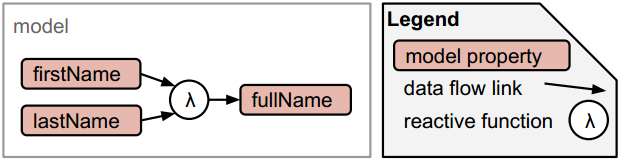
\includegraphics[width=\figureWidth]{figs/names.png}
  \caption [Full Name Reactive Model Example]{A basic reactive model that computes the full name whenever either the first name or last name changes. The reactive function is defined using the $when$ operator, therefore represents a node in a reactive data flow graph. }
  \label{fig:fullNameFlow}
\end{figure}

Lines 4 and 5 set a $when$ callback to log the full name whenever it changes. Lines 6 and 7 set the $firstName$ and $lastName$ properties on the $person$ model. This causes $fullName$ to be computed and set on the model. When $fullName$ is set, the callback that logs $fullName$ is invoked, causing the string \verb`"John Smith"` to be logged.

\section{Reactive Bar Chart} \label{reactiveBarChart}
Reactive models can serve as a foundation for interactive visualizations. Reactive models for multiple visualizations can be linked together at a higher level to form linked views. Interactive visualizations must respond to changes made by users such as resizing the display, changes in the data driving the visualization, changes in visualization configuration, and updates from other visualizations in a linked view context. This section introduces reactive visualization concepts through the example of a Bar Chart, then presents reusable reactive visualization components extracted from the Bar Chart.

A bar chart takes as input an array of data entries and a configuration that specifies the mapping from data attributes to the X and Y axes. It yields a dynamic bar chart graphic as output. The behavior desired for building the bar chart in response to changes in data and configuration fit perfectly within the framework of reactive models. As a first pass at constructing a reactive bar chart, the following reactive model properties are introduced:

\begin{itemize}
\item \verb`data` The input data table
\item \verb`xAttribute` The attribute used for the X scale (bar name)
\item \verb`yAttribute` The attribute used for the Y scale (bar height)
\end{itemize}

Using these three properties alone supports the essence of a bar chart, the plotting of bars and the labeling of axis tick marks. However, as attribute names are often cryptic and may not be the best labels for visualizations, two more model properties can be introduced that specify the text content of X and Y axis labels:

\begin{itemize}
\item \verb`xAxisLabel` The string displayed as the X axis label
\item \verb`yAxisLabel` The string displayed as the Y axis label
\end{itemize}

Bar charts and many other visualizations have an inner visualization rectangle in which visual marks are plotted. This inner rectangle lies within the outer rectangle containing the entire visualization, offset from the outer box by a specified margin. To integrate margin logic with reactive models, the following model properties are introduced:

\begin{itemize}
\item \verb`size` The size of the outer rectangle that contains the entire visualization, defined as an object with $width$ and $height$ properties in pixels.
\item \verb`margin` The margin object, having properties \verb`left`, \verb`right`, \verb`top` and \verb`bottom` in pixels, according to the D3 margin conventions \cite{d3conventionalmargins}.
\item \verb`width` The width of the inner visualization rectangle in pixels.
\item \verb`height` The height of the inner visualization rectangle in pixels.
\end{itemize}

The model properties defined this far support encapsulation of conventional D3 margins. A reactive function can be defined that updates $width$ and $height$ based on $size$ and $margin$. With the attributes present, scales can also be computed by reactive functions. The X scale depends on $data$, $xAttribute$, and $width$. The Y scale depends on $data$, $xAttribute$, and $height$. With the X and Y scales defined, the last remaining step is to compute the bars and axes from the data and scales. The complete reactive flow graph for a bar chart is shown in figure \ref{fig:barChartFlow}.

\begin{figure}
  \centering
  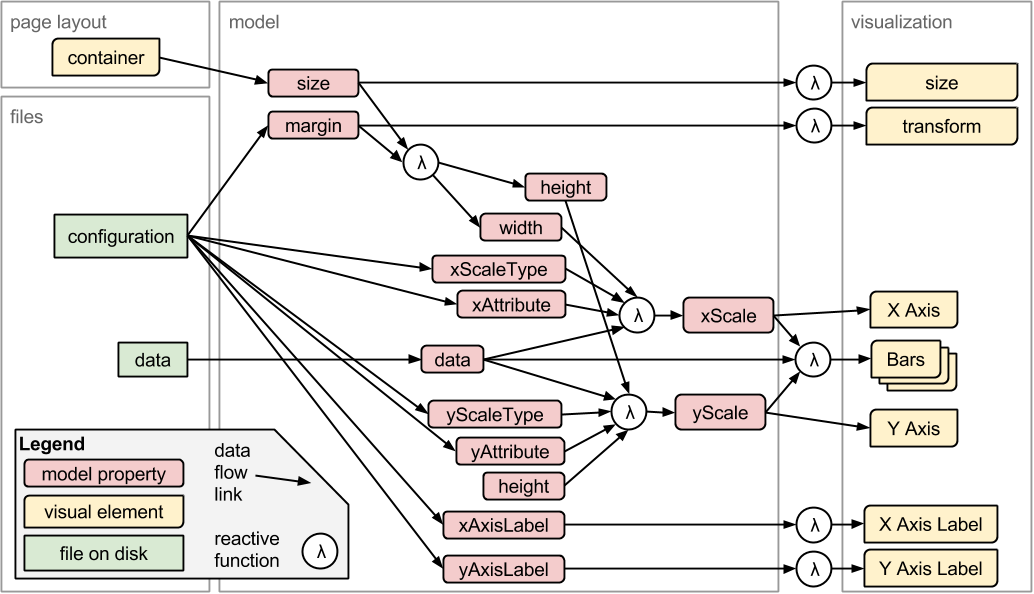
\includegraphics[width=\figureWidth]{figs/barChartFlow.png}
  \caption [Reactive Bar Chart Flow]{The data flow graph for a reactive bar chart based on \emph{reactive models}.}
  \label{fig:barChartFlow}
\end{figure}

\section{Reusable Reactive Flows}
Consider the following visualization techniques:
\begin{itemize}
\item Bar Chart
\item Scatter Plot
\item Line Chart
\item Stacked Area Chart
\end{itemize}

These visualizations share many underlying primitives such as scales, axes, and margins. The D3 Open Source project provides high quality generalized solutions for these and many more visualization primitives \cite{d3}. These visualization primitives and their computational dependency structure can be encapsulated by reactive flow graphs. Interactive forms of these visualizations also share interaction techniques for selecting visual marks such as rectangular brushing, hovering, clicking, panning, and zooming. Table \ref{table_components} lists reusable reactive flows common to many visualizations.

Other visualization techniques that may also be implemented using reactive models as a foundation include:

\begin{itemize}
\item Parallel Coordinates
\item Choropleth Map
\item Table
\item Box Plot
\end{itemize}

\newcommand{\diagramWidth}{1.9in}
\newcommand{\diagramScale}{0.4}
\newcommand{\descriptionWidth}{2.8in}
\newcommand{\descriptionPadding}{\vspace{.3\baselineskip}}

\begin{table*}
  \caption{Reusable flows for reactive visualization.}
  \centering
  \label{table_components}
  \begin{tabular}{ | c | c | c |}
    \hline
    \textbf{Component}
      & \textbf{Diagram}
      & \textbf{Description} \\ \hline
    margin
      & \parbox[c]{\diagramWidth}{\centering 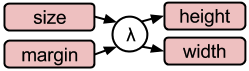
\includegraphics[scale=\diagramScale]{figs/margin.png}}
      & \parbox[c]{\descriptionWidth}{\descriptionPadding Computes the size of the inner visualization rectangle based on the container size (which may change when the user resizes the visualization) and the configured margin. \descriptionPadding}
      \\ \hline
    xScale
      & \parbox[c]{\diagramWidth}{\centering 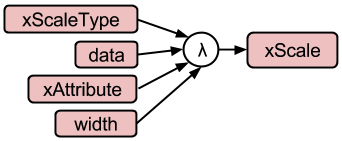
\includegraphics[scale=\diagramScale]{figs/xScale.png}}
      & \parbox[c]{\descriptionWidth}{ \descriptionPadding Computes the X scale. The domain is computed from the input data by evaluating the X attribute bounds. The range is computed from the inner visualization width. \descriptionPadding }
      \\ \hline
    xAxis
      & \parbox[c]{\diagramWidth}{\centering 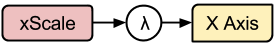
\includegraphics[scale=\diagramScale]{figs/xAxis.png}}
      & \parbox[c]{\descriptionWidth}{ \descriptionPadding Renders the X Axis (line, tick marks and labels) from the X scale \descriptionPadding.}
      \\ \hline
    xAxisLabel
      & \parbox[c]{\diagramWidth}{\centering 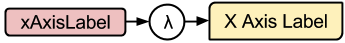
\includegraphics[scale=\diagramScale]{figs/xAxisLabel.png}}
      & \parbox[c]{\descriptionWidth}{ \descriptionPadding Renders the text label for the X Axis \descriptionPadding.}
      \\ \hline
    yScale
      & \parbox[c]{\diagramWidth}{\centering 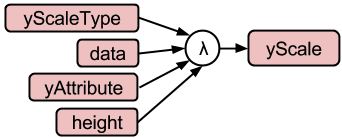
\includegraphics[scale=\diagramScale]{figs/yScale.png}}
      & \parbox[c]{\descriptionWidth}{ \descriptionPadding Computes the Y scale. The domain is computed from the input data by evaluating the Y attribute bounds. The range is computed from the inner visualization width. \descriptionPadding }
      \\ \hline
    yAxis
      & \parbox[c]{\diagramWidth}{\centering 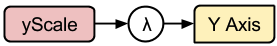
\includegraphics[scale=\diagramScale]{figs/yAxis.png}}
      & \parbox[c]{\descriptionWidth}{ \descriptionPadding Renders the Y Axis (line, tick marks and labels) from the Y scale \descriptionPadding.}
      \\ \hline
    yAxisLabel
      & \parbox[c]{\diagramWidth}{\centering 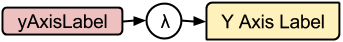
\includegraphics[scale=\diagramScale]{figs/yAxisLabel.png}}
      & \parbox[c]{\descriptionWidth}{ \descriptionPadding Renders the text label for the Y Axis \descriptionPadding.}
      \\ \hline
    colorScale
      & \parbox[c]{\diagramWidth}{\centering 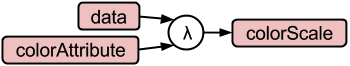
\includegraphics[scale=\diagramScale]{figs/colorScale.png}}
      & \parbox[c]{\descriptionWidth}{ \descriptionPadding Computes the color scale. The domain is computed from the input data by evaluating the set of unique values found in the color attribute. \descriptionPadding }
      \\ \hline
  \end{tabular}
\end{table*}

Property names serve as the common elements between components. Property names used in one or more components not introduced in the Bar Chart include:

\begin{itemize}
\item \verb1xScale1 The scale (domain and range) for the X axis.
\item \verb1xScaleType1 \verb1xScale1 qualifier: linear, logarithmic, or ordinal.
\item \verb1xAxis1 The visible X axis (tick marks and labels).

\item \verb1yScale1 The scale (domain and range) for the Y axis
\item \verb1yScaleType1 \verb1yScale1 qualifier: linear, logarithmic, or ordinal.
\item \verb1yAxis1 The visible Y axis (tick marks and labels).

\item \verb1colorAttribute1 The scale used to determine color of visual marks.
\item \verb1colorScale1 The scale used to determine color of marks.
\end{itemize}

Table \ref{table_components} lists components that can be combined to easily generate a foundation for a variety of interactive visualizations. These components encapsulate reusable reactive flows that implement the primitives necessary for interactive visualizations. Figure \ref{fig:barChartFlow} showed how several of these components can be assembled to create a general-purpose reactive bar chart. This bar chart flow represents a template for other visualizations, such as scatter plots. In fact, the only things that need to be changed in the bar chart flow to make it a scatter plot are (1) the X axis must be made quantitative, and (2) dots should be plotted rather than bars. Similarly, only the visual marks must be modified to change a scatter plot to a line chart, shown in figure \ref{fig:lineChart}.

\begin{figure}
  \centering
  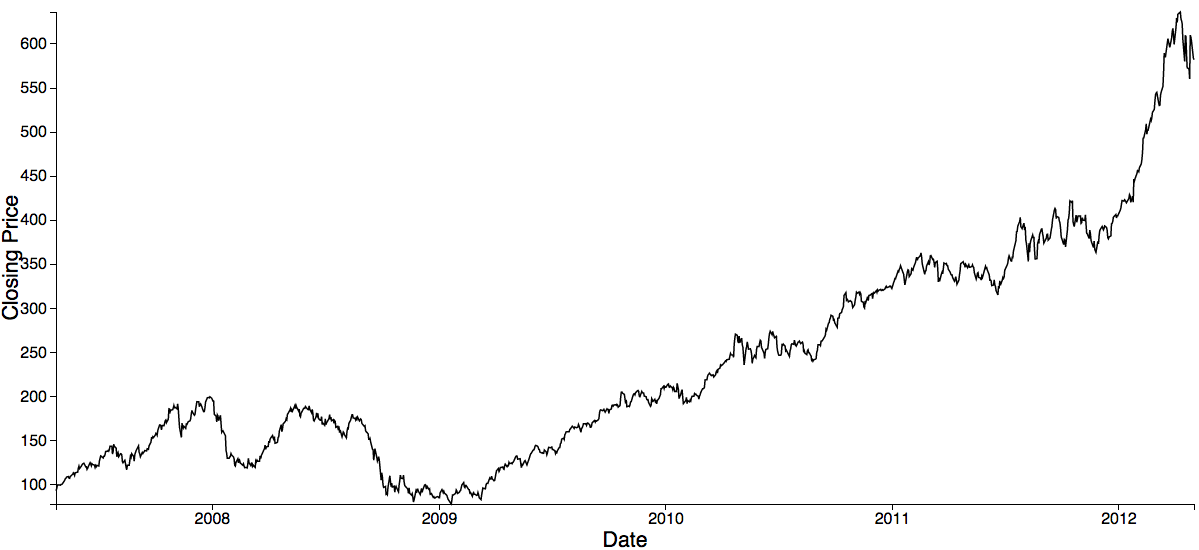
\includegraphics[width=\figureWidth]{figs/lineChart.png}
  \caption [Reactive Line Chart]{A line chart that shares scale and axis flows with scatter plots and bar charts.}
  \label{fig:lineChart}
\end{figure}

Interactive user interface components can be linked with any reactive model property. This makes it straightforward to add interactivity to reactive visualizations using conventional user interface elements such as dropdown menus, check boxes, sliders, and color pickers. For example, the X and Y attributes used by the scatter plot in figure \ref{fig:configurableScatter} can be made configurable using dropdown menus.

\begin{figure}
  \centering
  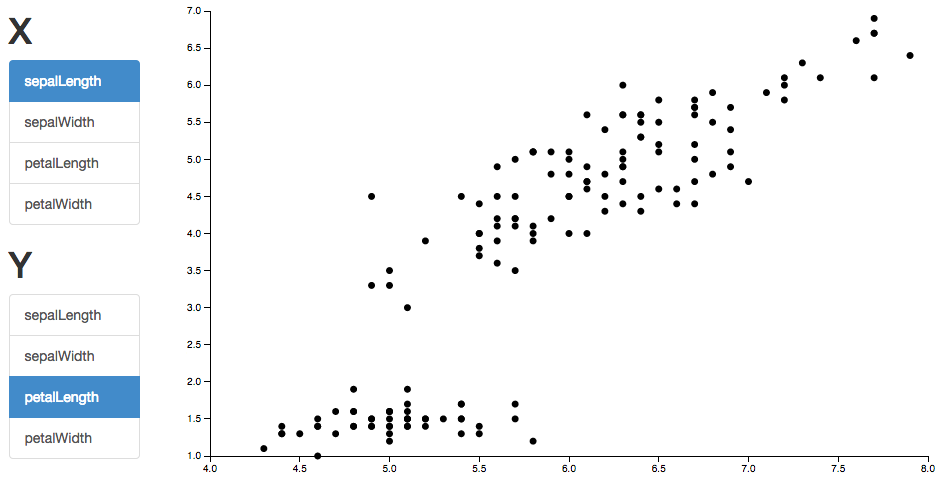
\includegraphics[width=\figureWidth]{figs/configurableScatter.png}
  \caption [Configurable Scatter Plot]{A scatter plot where X and Y attributes are selectable via Bootstrap List Group user interface elements.}
  \label{fig:configurableScatter}
\end{figure}
% and associated flow diagram.

% TODO include scatter plot flow diagram
% TODO make scatter plot flow diagram in Google Docs
% based on bar chart diagram.

% TODO automatically generate bar chart and scatter plot diagrams
\section{Linked Views}

Composing reactive visualizations from reusable flows yields reusable and composable interactive visualizations. Interactions such as brushing can be linked to the reactive model of the visualization instance. In the case of brushing, a model property \verb`brushedIntervals` contains the currently brushed intervals. This object stores the $(min, max)$ values for each attribute brushed. The updating brushed intervals can be used to as input to a filter operation that excludes data entries outside the brushed intervals. The output from the filter operator can be routed as input to another visualization. Figure \ref{fig:linkedViews} shows an example of linked views using this approach.

Figure \ref{fig:linkedViewsFlow} shows the overall flow of the linked scatter plot and bar chart. The brushing interaction sets a property on the reactive scatter plot called \verb1selectedData1. A reactive function that aggregates the selected data by Iris species links the selected data to the input data of the bar chart. Whenever the user brushes to select a new set of records in the scatter plot, the bar chart updates immediately to show only the selected data.

One advantage of reusable reactive flows is that when improvements are be made to a generalized feature, many visualizations manifest the improvement. For example, consider the X and Y axes used for many visualizations such as scatter plot and bar chart. The original D3 example that was drawn from to implement the axes had placed the axis labels inside the inner visualization rectangle. This had the unfortunate consequence that sometimes the label was occluded by marks within the visualization. To solve this issue, the axes were modified such that labels are placed outside the visualization area, are larger than tick mark labels, and are centered with respect to the axes. Figure \ref{fig:linkedViewsNew} shows the effect of the axis label improvement, which appears both in the scatter plot and bar chart.

\begin{figure}
  \centering
  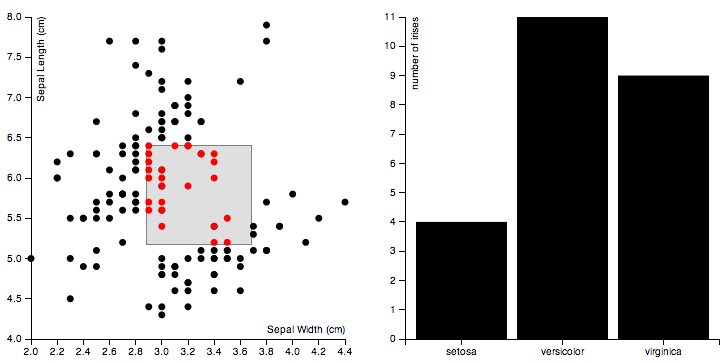
\includegraphics[width=\figureWidth]{figs/linkedViews.png}
  \caption [Linked Scatter Plot and Bar Chart]{A visualization of the Iris data set \cite{anderson1935irises} using linked views, powered by reactive visualization components. Brushing to select records in the scatter plot causes the selected data to be aggregated and displayed in the bar chart.}
  \label{fig:linkedViews}
\end{figure}

\begin{figure}
  \centering
  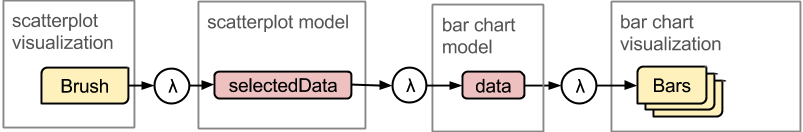
\includegraphics[width=\figureWidth]{figs/linkedViewsFlow.png}
  \caption [Linked Views Flow]{The (simplified) data flow graph for the linked scatter plot and bar chart example shown in figure \ref{fig:linkedViews}.}
  \label{fig:linkedViewsFlow}
\end{figure}

% TODO automatically generate linked view diagram

% TODO consider lazily evaluated model properties. Motivation: compute selected records from brush in scatter plot only when necessary.


\begin{figure}
  \centering
  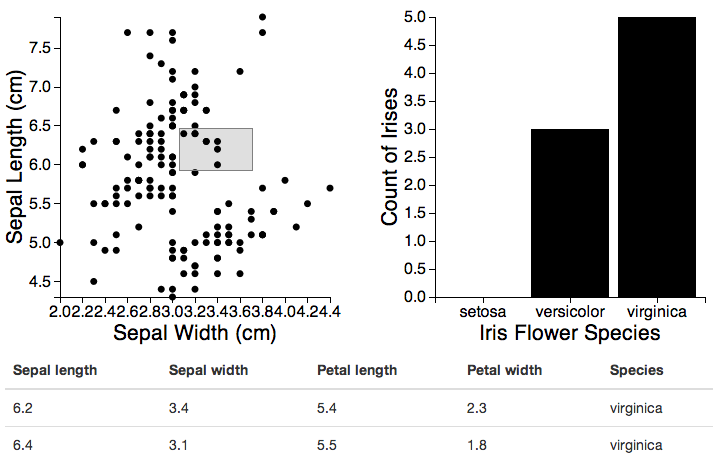
\includegraphics[width=\figureWidth]{figs/linkedViewsNew.png}
  \caption [Improved Linked Bar Chart, Scatter Plot and Table]{An improved version of the linked bar chart and scatter plot example. When changes are made in reusable components such as axes, the improvement is inherited by many reusable visualizations. This version also integrates with the reusable Bootstrap table component, showing the brushed selection in the table.}
  \label{fig:linkedViewsNew}
\end{figure}

\section{Summary}
This chapter introduced a novel way to combine elements of functional reactive programming with the Model View Controller (MVC) paradigm to create reactive models. Reactive models allow developers to specify data dependency graphs declaratively. This kind of abstraction is well suited for developing interactive visualizations because it drastically simplifies management of complex data flows and update patterns.

A collection of reusable reactive flows for interactive visualization was also introduced. These reactive flows encapsulate visualization primitives such as margins, scales, and axes. These flows were used as building blocks to generate a reusable bar chart, scatter plot and timeline. Visualizations with multiple linked views can be developed from these reusable visualization components in a straightforward manner .

\section{Future Work}
Future directions for this work will focus on developing a full catalog of reusable visualization components, coupling the data to currently available public data sources, visualization-centric user interfaces, and collaboration.

So far, the reactive visualization approach has been applied only to several visualization techniques. However, the following visualization techniques can also be supported:
\begin{itemize}
\item Color Legend
\item Pie Chart
\item Choropleth Map
\item Parallel Coordinates
\item Heatmap
\item Stacked Bar Chart
\item Stacked Area Chart
\item Streamgraph
\item TreeMap
\item Force Directed Graph Layout
\end{itemize}

Additionally, reusable components for the following interaction techniques can be encapsulated independently of any specific visualization technique using reactive models:
\begin{itemize}
\item Brushing - Dragging to define a selection region interactively.
\item Picking - Selecting a single visual mark by clicking or tapping on it.
\item Details-on-demand - A pattern of linked view composition in which an overview visualization can be used as navigation for a detailed view. This is a fundamental concept in interactive information visualization \cite{shneiderman1996eyes}.
\end{itemize}

A user interface for quickly assembling reusable components together based on graph drawing can also be developed. This user interface would show the data dependency diagrams similar to figure \ref{fig:barChartFlow}, but they would be dynamic and editable. Another direction for future research is integrating external user interface components such as traditional list selections, drop down menus, and radio buttons. One example of this concept is shown in figure \ref{fig:table}, which shows how reactive models can provide reactive HTML tables that can be linked with interactive visualizations. This would help in constructing intuitive user interfaces for manipulating the configuration of visualizations.

\begin{figure}
  \centering
  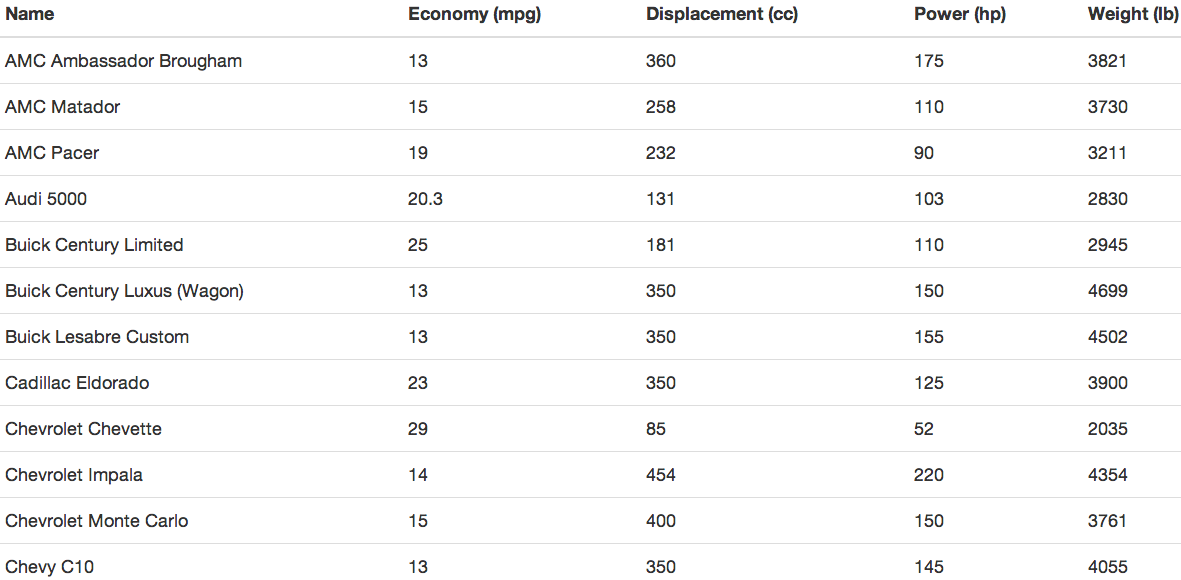
\includegraphics[width=\figureWidth]{figs/table.png}
  \caption [Reactive Table Visualization]{A visualization of the Cars data set \cite{hauser2002angular} by a reactive component that renders an HTML table style using Twitter Bootstrap \cite{lerner2012forge}.}
  \label{fig:table}
\end{figure}

